\documentclass[sigconf]{acmart}

\setcopyright{none}
\settopmatter{printacmref=true,printfolios=true}
\renewcommand\footnotetextcopyrightpermission[1]{}
\acmConference[MAS-GAIN '26]{2nd International Workshop on Multi-Agent Systems using Generative Artificial Intelligence for Automated Software Engineering}{October 2026}{Munich, Germany}
\acmBooktitle{2nd International Workshop on Multi-Agent Systems using Generative Artificial Intelligence for Automated Software Engineering (MAS-GAIN '26), October 2026, Munich, Germany}
\acmYear{2026}
\acmDOI{}
\acmISBN{}

\usepackage{booktabs}
\usepackage{multirow}
\usepackage{tabularx}
\usepackage{array}
\usepackage{tikz}
\usetikzlibrary{arrows.meta,positioning,fit,shapes.geometric}
\usepackage{xspace}
\emergencystretch=1em

\newcommand{\systemself}{\textsc{Self-Refine}\xspace}
\newcommand{\systemfree}{\textsc{Free-Form MAS}\xspace}
\newcommand{\systemstruct}{\textsc{Structured MAS}\xspace}

\title{Structured Evidence Handoffs in LLM Multi-Agent Vulnerability Analysis: Accuracy, Traceability, and Fault Propagation}

\author{Muhammad Umar Zeshan}
\affiliation{%
  \institution{University of L'Aquila}
  \city{L'Aquila}
  \country{Italy}
}
\email{muhammadumar.zeshan@student.univaq.it}

\begin{document}

\begin{abstract}
Multi-agent vulnerability analyzers often divide work among an analyst, a critic, and an adjudicator, yet it remains unclear whether structuring their communication improves the resulting security decisions. We report an exploratory controlled study of three matched workflows---single-agent self-refinement, a free-form analyst--refuter--adjudicator pipeline, and the same role pipeline using typed evidence records. All workflows use the same pinned Qwen2.5-Coder-3B model, code input, deterministic decoding, three calls, and generation ceilings. On 29 vulnerable--fixed C/C++ pairs from SecVulEval, the two multi-agent workflows achieved identical accuracy (51.7\%) and showed severe vulnerability over-prediction; an exact McNemar test found no paired accuracy difference ($p=1.0$). Structure nevertheless reduced completion tokens by 25.6\% and latency by 24.2\% relative to free-form collaboration, while making all 55 final claim references machine-traceable. A corrected 270-run fault-injection experiment revealed a trade-off: structured handoffs restored the pre-fault verdict in 96.7\% of verdict-inversion cases, but retained an injected false CWE in 93.3\% of evidence-corruption cases and copied the exact invalid span in 33.3\%. Thus, structured communication improved efficiency, lineage, and verdict stability, but could also preserve incorrect evidence more faithfully when verification was weak.
\end{abstract}

\keywords{multi-agent systems, large language models, vulnerability detection, evidence handoffs, fault injection, empirical software engineering}

\ccsdesc[500]{Computing methodologies~Multi-agent systems}
\ccsdesc[500]{Security and privacy~Software and application security}
\ccsdesc[300]{Software and its engineering~Software testing and debugging}

\maketitle

\section{Introduction}

Large language models (LLMs) are increasingly organized as multi-agent systems in which specialized roles exchange intermediate analyses before producing a final software-engineering decision. In security analysis, a natural decomposition assigns one agent to identify a candidate weakness, a second to challenge the evidence, and a third to adjudicate. Such designs promise cross-checking and auditability, but the additional messages also create new failure surfaces: evidence may be omitted, reformulated incorrectly, or propagated without verification.

Most evaluations obscure these process failures by reporting only the final task score. This is problematic because two systems can obtain the same accuracy while differing substantially in cost, traceability, and the path by which an error reaches the final verdict. Recent studies identify inter-agent misalignment and insufficient verification as recurring multi-agent failure modes~\cite{cemri2025mast}; software-engineering surveys similarly call for explicit interaction rules and process-level evaluation~\cite{he2025road}. Protocol-oriented work proposes structured messages as a remedy~\cite{mao2025semap}, while fault-injection studies show that architecture can change whether erroneous messages are challenged or silently propagated~\cite{huang2025resilience,jia2026masfire}. These findings motivate a narrower empirical question: \emph{what changes when vulnerability evidence is exchanged as typed records rather than free-form prose?}

Vulnerability analysis is a useful setting for this question. A plausible but unsupported security claim can be costly, and distinguishing a vulnerable function from its repaired counterpart is difficult for LLMs~\cite{ahmed2025secvuleval,wang2026vulagent}. Structured fields such as line spans, CWE identifiers, guard status, and claim provenance may improve auditability. They may also make a false claim easier to preserve mechanically.

We compare three workflows under matched inference conditions: (i) single-agent self-refinement, (ii) a free-form analyst--refuter--adjudicator system, and (iii) the same role pipeline using schema-constrained evidence handoffs. The main treatment contrast is the free-form versus structured representation; self-refinement provides a three-call baseline without distinct agent identities. We evaluate clean vulnerable--fixed discrimination, machine-checkable evidence lineage, efficiency, and response to controlled upstream faults.

The study addresses the following questions:

\begin{description}
  \item[RQ1:] How does communication structure influence the effectiveness and efficiency of agentic vulnerability analysis?
  \item[RQ2:] What evidence-integrity properties do structured handoffs provide across analyst, refuter, and adjudicator stages?
  \item[RQ3:] How does communication structure influence resilience to upstream verdict and evidence faults?
\end{description}

Our contributions are:
\begin{itemize}
  \item a role-matched comparison that holds the model, input, decoding policy, number of calls, and output ceilings constant while varying handoff representation;
  \item a process-level analysis separating end-task accuracy from efficiency, format reliability, claim traceability, and refuter behavior;
  \item a corrected 270-condition fault-injection experiment with matched verdict inversion, evidence deletion, and evidence corruption across all workflows; and
  \item an empirical trade-off: structured handoffs improve operational discipline and pre-fault verdict restoration, but can amplify the faithful propagation of false evidence.
\end{itemize}

Because prompt repair and eligibility screening were performed on the same development sample later used for measurement, we explicitly frame the results as exploratory rather than confirmatory.

\section{Background and Related Work}

\subsection{Multi-Agent Software Engineering}

LLM-based multi-agent systems use role specialization, iterative review, and orchestration to address software-engineering tasks. He et al. identify communication quality, conflict resolution, misinformation control, and evaluation beyond final artifacts as central research challenges~\cite{he2025road}. MAST empirically organizes multi-agent failures into system-design failures, inter-agent misalignment, and task-verification failures~\cite{cemri2025mast}. SEMAP responds with explicit behavioral contracts, structured messaging, and lifecycle verification~\cite{mao2025semap}. These studies motivate our focus on the representation and verification of intermediate evidence rather than on introducing another role architecture.

Self-Refine is an important baseline because one model generates an answer, critiques it, and revises it without additional training~\cite{madaan2023selfrefine}. Comparing this workflow with role-specialized agents helps separate the effect of distinct roles from the effect of spending three model calls.

\subsection{LLM-Based Vulnerability Analysis}

SecVulEval provides real-world C/C++ vulnerable and fixed functions with statement-level change information and reports that current LLMs remain weak at vulnerability localization with correct reasoning~\cite{ahmed2025secvuleval}. GPTLens separates generation and discrimination to reduce false positives in smart-contract auditing~\cite{hu2023gptlens}. VulAgent uses hypothesis generation and validation for project-level vulnerability analysis~\cite{wang2026vulagent}. MulVul combines a retrieval-augmented router with specialized detector agents and cross-model prompt evolution~\cite{wu2026mulvul}. LAMPS demonstrates role-specialized multi-agent reasoning for malicious-package detection~\cite{zeshan2026lamps}. Collectively, this work establishes that critic and validator roles are common in agentic security analysis. Our contribution is not the first multi-agent detector; it is the controlled isolation of handoff format and the measurement of evidence propagation.

\subsection{Fault Injection and Resilience}

Huang et al. inject faulty agent messages and show that challenge and inspection mechanisms can improve resilience~\cite{huang2025resilience}. MAS-FIRE systematizes intra-agent and inter-agent fault types and evaluates how architectures recover from modified prompts, responses, and routing~\cite{jia2026masfire}. We adapt this idea to vulnerability evidence. The injected conditions target a verdict, the availability of supporting evidence, or a concrete false claim and location. Unlike end-task-only evaluation, our analysis records whether the injected content appears in the final report.

The closest conceptual expectation is that structure should reduce ambiguity and make verification easier. The competing expectation is that schema-compliant misinformation may be treated as authoritative. Our experiment tests both possibilities.

\section{Study Design}

\subsection{Dataset and Eligibility}

We use vulnerable--fixed C/C++ function pairs prepared from SecVulEval~\cite{ahmed2025secvuleval}. The deterministic preparation configuration used seed 20260712, retained at most one pair per project, and accepted functions containing 4--300 lines and at most 12,000 characters. The development split contained 30 pairs. One pair (CVE-2020-15861, CWE-59) was excluded after a function-only eligibility audit: the security-relevant filesystem and symbolic-link behavior was implemented in unseen callees, while the supplied function exposed only calls to those helpers. The measured clean sample therefore contains 29 projects, 58 code versions, and 174 workflow executions.

The agents receive only the numbered function body. Project names, labels, CVE/CWE metadata, commit messages, and changed-line annotations are withheld. The fixed counterpart is interpreted as the version in which the target vulnerability was reportedly repaired, not as globally vulnerability-free. Changed lines are used only as a localization proxy.

\subsection{Compared Workflows}

Figure~\ref{fig:workflows} summarizes the three workflows.

\begin{figure*}[t]
  \centering
  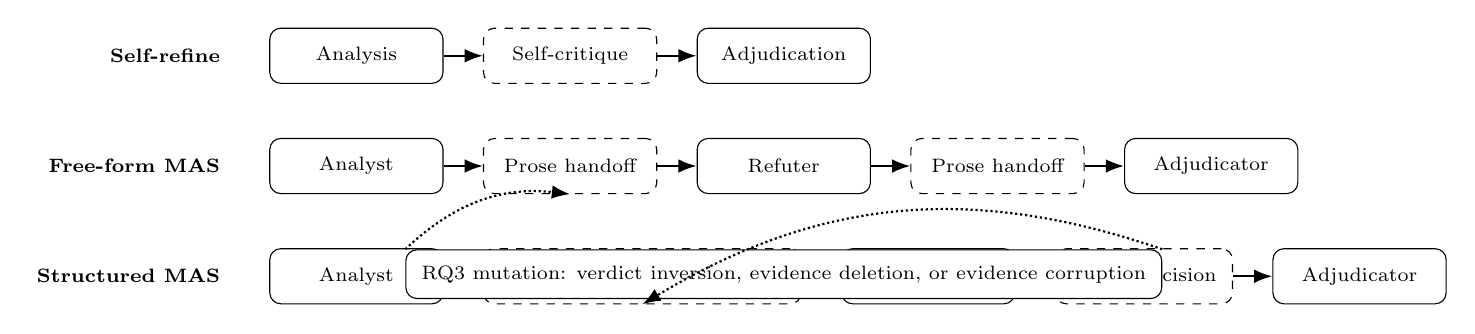
\begin{tikzpicture}[
  font=\scriptsize,
  node distance=4mm and 5mm,
  box/.style={draw,rounded corners,minimum height=7mm,minimum width=22mm,align=center,inner sep=2mm},
  hand/.style={draw,dashed,rounded corners,minimum height=7mm,minimum width=22mm,align=center,inner sep=2mm},
  arr/.style={-Latex,thick},
  label/.style={font=\bfseries\scriptsize,anchor=east}
]
\node[label] (l1) at (0,1.4) {Self-refine};
\node[box,right=5mm of l1] (s1) {Analysis};
\node[hand,right=of s1] (s2) {Self-critique};
\node[box,right=of s2] (s3) {Adjudication};
\draw[arr] (s1)--(s2); \draw[arr] (s2)--(s3);

\node[label] (l2) at (0,0) {Free-form MAS};
\node[box,right=5mm of l2] (f1) {Analyst};
\node[hand,right=of f1] (f2) {Prose handoff};
\node[box,right=of f2] (f3) {Refuter};
\node[hand,right=of f3] (f4) {Prose handoff};
\node[box,right=of f4] (f5) {Adjudicator};
\draw[arr] (f1)--(f2); \draw[arr] (f2)--(f3); \draw[arr] (f3)--(f4); \draw[arr] (f4)--(f5);

\node[label] (l3) at (0,-1.4) {Structured MAS};
\node[box,right=5mm of l3] (t1) {Analyst};
\node[hand,right=of t1] (t2) {Typed claim: ID, span, CWE};
\node[box,right=of t2] (t3) {Refuter};
\node[hand,right=of t3] (t4) {Typed decision};
\node[box,right=of t4] (t5) {Adjudicator};
\draw[arr] (t1)--(t2); \draw[arr] (t2)--(t3); \draw[arr] (t3)--(t4); \draw[arr] (t4)--(t5);

\node[draw,fill=white,rounded corners,align=center,inner sep=2mm,below=7mm of f3] (fault) {RQ3 mutation: verdict inversion, evidence deletion, or evidence corruption};
\draw[-Latex,densely dotted,thick] (fault.north west) to[bend left=25] (f2.south);
\draw[-Latex,densely dotted,thick] (fault.north east) to[bend right=25] (t2.south);
\end{tikzpicture}

  \Description{Three matched three-call workflows: self-refinement, free-form analyst-refuter-adjudicator, and structured analyst-refuter-adjudicator, with upstream fault injection before the critique or refutation stage.}
  \caption{Matched three-call workflows and the corrected fault-injection point. Free-form and structured MAS use identical roles; only the handoff representation differs.}
  \label{fig:workflows}
\end{figure*}

\textbf{Self-refinement} uses one model identity for initial analysis, critique, and final adjudication. \textbf{Free-form MAS} uses analyst, refuter, and adjudicator roles exchanging prose. \textbf{Structured MAS} uses the same three roles, but the analyst emits a typed claim containing an identifier, statement, optional line span and CWE, source/sink information, guard status, consequence, and confidence. The refuter returns a decision for the claim, and each final finding names its source claim.

All workflows use Qwen2.5-Coder-3B-Instruct~\cite{hui2024qwen25coder}, pinned to revision \texttt{488639f1ff808d1d3d0ba301aef8c11461451ec5}. Inference uses Transformers with 4-bit loading on an NVIDIA T4, an 8,192-token input limit, and deterministic greedy decoding (\texttt{do\_sample=false}). Each workflow makes three calls with stage ceilings of 340, 220, and 480 completion tokens. Final reports share one strict JSON schema. A malformed final report counts as failure rather than being rescued by keyword heuristics.

\subsection{Protocol Development}

An initial 30-pair pilot exposed verbosity and JSON truncation, especially in adjudication. We reduced each report to at most one principal claim/finding, constrained spans and CWE enumeration, and redistributed the fixed 1,040-token completion ceiling. A 10-pair failure-focused stress subset was used to validate the repaired protocol. We then froze the prompts and budgets before the 29-pair clean run. This procedure improves execution reliability but makes the reported sample development data; Section~\ref{sec:threats} discusses the resulting validity limitation.

\subsection{Measures and Analysis}

For \textbf{RQ1}, version accuracy is the proportion of vulnerable and fixed functions classified correctly. Pair correctness requires both versions of a pair to be correct. We additionally report vulnerable recall, fixed-version accuracy, false-positive rate, completion tokens, latency, and parsing failures. We use Cochran's $Q$ for the three paired workflows, exact McNemar tests for pairwise correctness~\cite{cochran1950,mcnemar1947}, and paired Wilcoxon signed-rank tests for efficiency~\cite{wilcoxon1945}; pairwise $p$-values are Holm-adjusted where stated~\cite{holm1979}.

For \textbf{RQ2}, the structured records permit automatic checks of claim-ID lineage, unsupported final references, parser validity, and refuter decisions. These are integrity and auditability measures, not a substitute for human judgment of semantic correctness.

For \textbf{RQ3}, we deterministically selected the first 15 lexicographically sorted eligible pair IDs (30 versions). We reused each clean upstream analysis, converted it into a canonical one-claim representation, and injected three faults before rerunning only the critic/refuter and adjudicator:
\begin{itemize}
  \item \emph{verdict inversion}: replace the upstream verdict with its opposite; an uncertain verdict is deterministically replaced with vulnerable;
  \item \emph{evidence deletion}: retain the verdict but remove all claims and supporting evidence; and
  \item \emph{evidence corruption}: replace the support with a fabricated CWE-787 claim and a span 50--51 lines beyond the function.
\end{itemize}
For prose workflows, the mutated record is serialized into canonical text; Structured MAS receives the equivalent JSON. The 270 resulting records comprise $15\times2\times3\times3$ conditions. Direct propagation measures include restoration of the pre-fault verdict, following the injected verdict, retaining CWE-787, and copying the exact invalid span. Wilson intervals accompany key proportions.

\section{Results}

\subsection{RQ1: Effectiveness and Efficiency}

Table~\ref{tab:rq1} reports the clean-run results. None of the workflows performs materially above chance. Free-form and Structured MAS both classify 30 of 58 versions correctly (51.7\%), while self-refinement classifies 28 (48.3\%). Cochran's test finds no overall difference ($Q=0.62$, $p=.735$). Free-form and Structured MAS agree on 54 of 58 predictions (93.1\%). In the four disagreements, each is uniquely correct twice; exact McNemar testing therefore returns $p=1.0$.

\begin{table}[t]
\centering
\caption{Clean results over 29 vulnerable--fixed pairs. Values are percentages except tokens and seconds.}
\label{tab:rq1}
\setlength{\tabcolsep}{3.2pt}
\begin{tabular}{lrrr}
\toprule
Metric & Self & Free & Structured \\
\midrule
Accuracy & 48.3 & 51.7 & 51.7 \\
Vulnerable recall & 79.3 & 96.6 & 96.6 \\
Fixed accuracy & 17.2 & 6.9 & 6.9 \\
False-positive rate & 82.8 & 93.1 & 93.1 \\
Pair correctness & 10.3 & 6.9 & 3.4 \\
Final parse failures & 0 & 0 & 0 \\
Mean completion tokens & 708.8 & 714.9 & \textbf{532.0} \\
Mean latency (s) & 62.2 & 62.6 & \textbf{47.4} \\
\bottomrule
\end{tabular}
\end{table}

The aggregate accuracy hides a severe class bias. Free-form and Structured MAS correctly identify 28 of 29 vulnerable versions, but label 27 of 29 fixed versions as vulnerable. Self-refinement is slightly less extreme, correctly identifying 23 vulnerable and five fixed versions. Pair correctness is consequently low: three pairs for self-refinement, two for free-form, and one for structured communication.

Structure does produce a clear efficiency difference. Structured MAS uses 25.6\% fewer completion tokens and 24.2\% less mean latency than Free-form MAS. Paired Wilcoxon tests are significant for both completion tokens ($p<10^{-9}$) and latency ($p<10^{-9}$). It is similarly cheaper than self-refinement, while free-form and self-refinement do not differ significantly in either measure.

\noindent\textbf{Answer to RQ1.} Communication structure did not improve classification effectiveness in this sample. It did improve operational efficiency: the structured workflow reached the same version accuracy as free-form collaboration with substantially fewer generated tokens and lower latency.

\subsection{RQ2: Evidence Integrity}

Table~\ref{tab:rq2} summarizes the typed evidence trail. Structured MAS produced 56 analyst claims across 58 records, 58 refuter decisions, and 55 final findings. Every final source-claim reference matched an analyst claim, and no unsupported claim ID appeared. All three structured stages parsed successfully.

\begin{table}[t]
\centering
\caption{Machine-checkable evidence integrity in Structured MAS.}
\label{tab:rq2}
\setlength{\tabcolsep}{4pt}
\begin{tabular}{lr}
\toprule
Measure & Count / rate \\
\midrule
Analyst claims & 56 \\
Refuter decisions & 58 \\
Final findings & 55 \\
Traceable final claim references & 55/55 (100\%) \\
Unsupported final claim references & 0/55 (0\%) \\
Supported decisions & 57/58 (98.3\%) \\
Refuted decisions & 1/58 (1.7\%) \\
Corrected or uncertain decisions & 0/58 (0\%) \\
Stage parse failures & 0/174 (0\%) \\
\bottomrule
\end{tabular}
\end{table}

This is strong syntactic integrity but weak evidence of substantive challenge. The refuter supports 57 of 58 decisions, refutes only one, and never issues a correction or an uncertain decision. Moreover, complete lineage coexists with the poor fixed-version accuracy in Table~\ref{tab:rq1}. Machine-checkable provenance therefore shows where a claim came from, not whether it is correct.

\noindent\textbf{Answer to RQ2.} Typed handoffs made final evidence lineage complete and automatically auditable, with no unsupported identifiers or parsing failures. They did not induce meaningful skepticism: almost every upstream claim was supported, including many claims that led to false positives.

\subsection{RQ3: Resilience to Upstream Faults}

Of the 270 corrected fault runs, 269 produced valid final reports. Three downstream stages reported parse errors: two structured refuter outputs were replaced by the protocol fallback and still yielded valid final reports, while one structured adjudication under verdict inversion remained invalid. Table~\ref{tab:rq3} separates the three fault mechanisms; task accuracy under each fault is included for context, but propagation measures are more diagnostic.

\begin{table*}[t]
\centering
\caption{Corrected fault-injection outcomes on 30 versions per system and fault. Gold overlap uses SecVulEval changed lines as a localization proxy.}
\label{tab:rq3}
\setlength{\tabcolsep}{4.2pt}
\begin{tabular}{llrrr}
\toprule
Fault & Outcome & Self & Free & Structured \\
\midrule
\multirow{3}{*}{Verdict inversion}
 & Pre-fault verdict restored & 83.3 & 43.3 & \textbf{96.7} \\
 & Injected verdict followed & 10.0 & 26.7 & \textbf{0.0} \\
 & Task accuracy & 53.3 & 43.3 & 50.0 \\
\midrule
\multirow{3}{*}{Evidence deletion}
 & Final finding generated & 53.3 & 26.7 & \textbf{100.0} \\
 & Final span overlaps gold proxy & 26.7 & 13.3 & \textbf{50.0} \\
 & Task accuracy & 43.3 & 43.3 & 50.0 \\
\midrule
\multirow{3}{*}{Evidence corruption}
 & Injected CWE-787 retained & 20.0 & 23.3 & \textbf{93.3} \\
 & Exact invalid span copied & 10.0 & 10.0 & \textbf{33.3} \\
 & Task accuracy & 43.3 & 53.3 & 43.3 \\
\bottomrule
\end{tabular}
\end{table*}

For verdict inversion, Structured MAS restores the pre-fault verdict in 29 of 30 cases (96.7\%, 95\% Wilson CI [83.3, 99.4]) and never follows the injected verdict. Free-form MAS restores only 13 of 30 (43.3\%, CI [27.4, 60.8]). The free-form--structured difference is significant under exact McNemar testing after Holm correction ($p_{\mathrm{adj}}<.001$). Self-refinement also restores the pre-fault verdict frequently (83.3\%), and its difference from Structured MAS is not significant.

Evidence deletion produces a different behavior. Structured MAS generates a final finding and span in all 30 cases even though all upstream claims were removed; 15 spans overlap the changed-line proxy. Free-form and self-refinement generate findings less often. This may be recovery through rereading the code, but it may also be unsupported reconstruction. None of the systems abstains consistently.

Evidence corruption reveals the central failure mode. Structured MAS retains the standardized false CWE-787 claim in 28 of 30 final reports (93.3\%, CI [78.7, 98.2]), compared with seven free-form and six self-refinement reports. The free-form--structured paired difference remains significant after Holm correction ($p_{\mathrm{adj}}<.001$). Structured MAS also copies the exact out-of-range line span in 10 cases, versus three for each alternative, although this span difference does not remain significant after adjustment. Internally, the structured refuter supports the corrupted claim in 24 cases and refutes it in six.

\noindent\textbf{Answer to RQ3.} Structure strongly stabilized the categorical verdict against direct inversion, but it also made semantically corrupted evidence more persistent. The same lineage mechanism that reliably preserved a decision frequently preserved a false CWE and invalid location when the refuter failed to verify them.

\section{Discussion}

\subsection{Structure Changes the Process, Not Necessarily the Decision}

The clean comparison separates three effects that aggregate accuracy alone would conflate. First, the two MAS variants have equal accuracy but are not identical: they disagree on four cases, with two unique successes each. Second, the structured workflow is substantially cheaper. Its constrained messages reduce generation without a corresponding accuracy loss. Third, typed evidence creates complete claim lineage. The treatment therefore changes how the system operates even when it does not shift the final classification boundary.

This distinction matters for multi-agent evaluation. A paper that reports only accuracy would conclude that the two MAS designs are equivalent. A process-level evaluation instead shows that one is more compact and auditable, while neither solves the underlying model's tendency to label repaired code as vulnerable. The very low pair correctness is especially important: high vulnerable recall is achieved by predicting vulnerability for almost every version.

\subsection{Traceability Is Not Verification}

The RQ2 and RQ3 results jointly expose a limitation of structured communication. All final structured claim references are valid, yet the refuter approves 98.3\% of clean claims and 80\% of corrupted-evidence claims. The schema guarantees that a final finding can point to an upstream claim; it does not guarantee that the claim's line range exists or that its CWE follows from the code.

This leads to a practical design principle: \emph{lineage should be paired with independent evidence validation}. A production analyzer should reject out-of-range spans before the next agent sees them, require the refuter to quote counter-evidence, and separate ``schema-valid'' from ``evidence-valid.'' A verifier could deterministically check line bounds and use static analysis, retrieval, tests, or a distinct model to validate source-to-sink paths. Without such mechanisms, structure can make misinformation look authoritative.

\subsection{Fault-Specific Resilience}

The structured pipeline is not uniformly robust or fragile. It resists a direct verdict flip because the downstream stages reread the code and can restore the previous categorical decision. In contrast, a detailed false claim supplies a plausible narrative, CWE, confidence, and location that the structured refuter often accepts. Resilience therefore depends on the fault's semantic depth. Protecting a single label is easier than invalidating a well-formed but unsupported explanation.

The evidence-deletion condition further cautions against treating non-abstention as success. Structured MAS always reconstructs a finding, but only half of the spans overlap the changed-line proxy. In security analysis, confident reconstruction from missing evidence may be more dangerous than an explicit ``insufficient evidence'' response.

\subsection{Implications for MAS-GAIN Research}

The results support evaluating agentic software-engineering systems along at least four axes: task outcome, efficiency, communication integrity, and fault containment. Structured protocols are valuable engineering mechanisms, but their benefits should not be inferred from format compliance. Benchmarks should retain stage-level traces, distinguish refutation from repetition, and inject semantic faults that remain valid at the message-schema level. Negative results are also informative: adding roles and structure did not overcome the base model's false-positive bias in this function-only setting.

\section{Threats to Validity}
\label{sec:threats}

\textbf{Internal validity.} The protocol was repaired after observing truncation on the 30-pair development split, and the final clean run reused 29 of those pairs. The study is therefore exploratory and may overestimate formatting reliability. The function-only eligibility exclusion was also made after the pilot exposed repeated failures, although the stated reason---security behavior implemented in unseen callees---is independent of the model's predicted label. We disclose the pair and exclusion rule rather than presenting the sample as held out.

\textbf{Construct validity.} Changed lines are a proxy for vulnerability localization, not exact root-cause ground truth. The RQ2 analysis measures syntactic lineage and refuter decisions; it does not include independent human annotation of semantic preservation. A traceable claim can be false, as RQ3 demonstrates. ``Pre-fault verdict restoration'' measures stability relative to the clean upstream handoff, not correctness relative to the dataset.

\textbf{RQ3 validity.} To apply matched mutations, free-form and self-refinement outputs were canonicalized into a common one-claim text representation, whereas Structured MAS received equivalent JSON. We did not run a no-fault canonicalized control, so fault-condition task-accuracy changes may include a representation effect. We therefore emphasize direct propagation measures such as retained CWE and exact span. Mapping an uncertain verdict to vulnerable during inversion is deterministic but asymmetric.

\textbf{External validity.} The experiment uses one 3B open-weight code model, one deterministic run, 29 C/C++ projects, and function-only context. Results may differ for larger or proprietary models, repository-level tools, other languages, or multi-agent systems with memory and tool use. Agent identities are prompt-defined instances of the same model rather than independently trained agents.

\textbf{Conclusion validity.} The sample is small, especially for 30-condition fault comparisons. We use paired tests and Wilson intervals, but absence of significance is not equivalence. Multiple comparisons are Holm-adjusted when used for principal claims. Runtime was measured on a shared Colab T4 environment and should be interpreted comparatively rather than as an absolute deployment benchmark.

\section{Conclusion}

We investigated whether typed evidence handoffs improve LLM-based multi-agent vulnerability analysis. On 29 vulnerable--fixed pairs, structured and free-form collaboration achieved the same 51.7\% accuracy and shared a severe false-positive bias. Structure nevertheless reduced generated tokens and latency and provided complete machine-checkable claim lineage. Under controlled faults, it almost always restored an inverted upstream verdict, yet it also retained a standardized false CWE in 93.3\% of cases and copied invalid locations more often than the alternatives.

The central lesson is that structured communication is an amplifier of process discipline, not an assurance of evidence quality. It can make correct information easier to preserve and inspect, but it can also make a plausible false claim easier to propagate. Reliable agentic security analysis therefore requires schemas plus independent verification, bounded abstention, and benchmarks that examine the trajectory of evidence rather than only the final verdict.


\bibliographystyle{ACM-Reference-Format}
\bibliography{references}

\end{document}
